% !TEX program = xelatex
% RAI Risk Taxonomy Technical Report 2.0, Korean current release edition.
\documentclass[11pt,a4paper]{article}
\usepackage[a4paper,top=22mm,bottom=24mm,left=22mm,right=22mm]{geometry}
\usepackage{fontspec}
\usepackage{microtype}
\usepackage{booktabs,tabularx,array}
\usepackage{enumitem}
\usepackage{amsmath,amssymb}
\usepackage{seqsplit}
\usepackage{graphicx}
\usepackage{float}
\usepackage{pgfplots}
\usepackage{fancyhdr}
\usepackage[hidelinks]{hyperref}
\pgfplotsset{compat=1.18}

\IfFileExists{/System/Library/Fonts/AppleSDGothicNeo.ttc}{%
  \setmainfont{Apple SD Gothic Neo}\setsansfont{Apple SD Gothic Neo}\setmonofont{Menlo}%
}{%
  \setmainfont{Noto Sans CJK KR}\setsansfont{Noto Sans CJK KR}\setmonofont{Noto Sans Mono CJK KR}%
}
\newcommand{\code}[1]{\texttt{#1}}
\newcolumntype{Y}{>{\raggedright\arraybackslash}X}
\newcolumntype{L}[1]{>{\raggedright\arraybackslash}p{#1}}
\setlength{\parindent}{1.2em}
\setlength{\parskip}{0pt}
\setlength{\emergencystretch}{2em}

\definecolor{natureblue}{HTML}{0072B2}
\pgfplotsset{
  natureaxis/.style={
    axis x line*=bottom,
    axis y line*=left,
    axis line style={black, line width=0.6pt},
    tick align=outside,
    tick style={black, line width=0.5pt},
    tick label style={font=\sffamily\footnotesize, color=black},
    label style={font=\sffamily\small, color=black},
    grid=none,
    clip=false
  }
}

\pagestyle{fancy}
\setlength{\headheight}{14pt}
\fancyhf{}
\lhead{\footnotesize RAI Risk Taxonomy}
\rhead{\footnotesize Technical Report 2.0}
\cfoot{\footnotesize\thepage}

\begin{document}

\begin{center}
{\LARGE\bfseries RAI Risk Taxonomy 2.0\par}
\vspace{4pt}
{\large 현행 계층, 재현 가능한 매핑 및 신뢰성 검증\par}
\vspace{8pt}
{\large RAI Risk Taxonomy Project\par}
\vspace{2pt}
2026년 7월 25일 \,·\, release candidate v2.18.0-rc
\end{center}

\begin{abstract}
\noindent
RAI Risk Taxonomy 2.0은 General-purpose AI, Agentic AI, Physical AI의
책임 AI 리스크를 통합한다. 현행 릴리스는 등록 ID 1,711개를 보존하면서 독립된
활성 L4 카드 1,660개와 통합 이력 51개를 구분한다. 표준 기반 상위 구조와 문헌
기반 L4 발굴을 결합한 Hybrid 접근을 사용했으며, 현재 계층은 의미 L2 3개와
의미 L3 54개로 구성된다. General AI에는 사회적 파급 관련 L3 4개를 신설했고,
기존 Physical AI의 사회적 영향 L3 9개는 General 사회적 파급 아래로 이동했다.
L4 배치는 BGE-M3 임베딩, L3 정의, 군집 중심점, 키워드 유사도 및 도메인 제약을
결합해 수행한다. 입력 파일 해시, 모델 스냅샷, 난수 시드, 반복 이력 및 불변조건
검사를 통해 재현성을 관리한다. 활성 카드 전체에서 구면 EM은 20회에 수렴했고
평균 코사인 목적함수는 0.8005였다. Top-1 일치율은 71.9\%, Top-5 일치율은
95.2\%였다. 본 보고서는 현재 결과와 재현 절차를 중심으로 기술하며, 경계 사례는
후속 휴먼 검토 대상으로 유지한다.
\end{abstract}

\section{범위와 설계 목표}

AI 리스크는 텍스트 유해성에서 자율적 행동, 도구 사용, 다중 에이전트 상호작용,
물리 세계 영향으로 확장되고 있다. 분류체계는 L0부터 L4까지의 5계위 구조를
사용한다. L1은 기술 도메인, L2는 공통 안전 차원, L3는 리스크군, L4는 구체적인
위험 메커니즘을 나타낸다.

등록 ID와 분석 단위를 구분한다. ID 레지스트리는 1,711개로 고정하며, 이 중
1,660개는 독립된 활성 카드, 51개는 인용 및 출처 추적을 위해 보존하는 통합
이력이다. 별도 표시가 없는 모든 계층 통계와 신뢰성 검증은 활성 카드 1,660개를
기준으로 한다.

\section{근거자료와 ID 레지스트리}

\begin{table}[H]
\centering
\caption{근거자료에서 현행 분류체계까지의 단계별 집계}
\small
\begin{tabularx}{\linewidth}{L{0.24\linewidth}r L{0.18\linewidth}Y}
\toprule
단계 & 수량 & 단위 & 주요 포함 기준 \\
\midrule
전체 AI 근거자료 & 3,906,767 & 문헌 또는 특허 & AI 자료원, 유효 제목, 표준 스키마, 유형 내 중복 제거 \\
AI 리스크 근거자료 & 82,971 & 문헌 또는 특허 & 검토된 리스크 자료원과 문서 유형 필터 \\
완전일치 중복 제거 후보 & 1,725 & 카드 후보 & 정규화된 명칭과 핵심 정의의 완전일치 \\
등록 L4 ID & 1,711 & 식별자 & 계층명 누출 제거, 모든 ID 이력 보존 \\
활성 L4 카드 & 1,660 & 독립 카드 & 통합 이력 51개를 활성 분석에서 제외 \\
\bottomrule
\end{tabularx}
\end{table}

현행 빌드는 모든 ID의 유일성, 통합 이력의 활성 카드 연결, 모든 활성 카드의
주 경로와 의미 L3 경로 존재, 통합 이력의 활성 통계 제외를 불변조건으로
검사한다.

\section{현행 계층과 커버리지}

의미 L2는 Interaction Safety, System Safety, Societal Impact의 3개다.
현재 의미 L3는 General 33개, Agentic 6개, Physical 15개로 총 54개다.
General 사회적 파급에는 에너지 소비 및 환경 오염, 책임성 부족 및 거버넌스
체계 부재, 투명성 부족, 공정성의 L3 4개를 신설했다. 기존 Physical 사회적
영향 L3 9개는 General 사회적 파급 아래로 이동했다.

\begin{table}[H]
\centering
\caption{L1 도메인별 현행 커버리지}
\begin{tabular}{lrrr}
\toprule
L1 도메인 & 의미 L3 & 활성 주 경로 L4 & 활성 L4 비중 \\
\midrule
General-purpose AI & 33 & 1,221 & 73.6\% \\
Agentic AI & 6 & 281 & 16.9\% \\
Physical AI & 15 & 158 & 9.5\% \\
\midrule
합계 & 54 & 1,660 & 100.0\% \\
\bottomrule
\end{tabular}
\end{table}

\begin{table}[H]
\centering
\caption{의미 L1 및 L2 경로별 활성 L4 카드}
\begin{tabular}{lrrrr}
\toprule
L1 도메인 & Interaction & System & Societal Impact & 합계 \\
\midrule
General-purpose AI & 641 & 467 & 108 & 1,216 \\
Agentic AI & 0 & 286 & 0 & 286 \\
Physical AI & 64 & 94 & 0 & 158 \\
\midrule
합계 & 705 & 847 & 108 & 1,660 \\
\bottomrule
\end{tabular}
\end{table}

첫 번째 표는 홈페이지의 주 탐색 경로를 집계한다. 두 번째 표는 경계 검토 카드의
보존된 의미 경로를 사용한다. 이 때문에 General과 Agentic의 도메인 수에는
5건의 차이가 있으나 전체 합계는 동일하다. 모든 활성 카드는 의미 L3 경로를
가지며, 54개 L3 모두 비어 있지 않다. 가장 큰 L3는 Anthropomorphism 160건으로
전체의 9.6\%이며, 상위 5개 L3는 553건으로 33.3\%다.

\begin{figure}[H]
\centering
\begin{tikzpicture}
\begin{axis}[
  natureaxis,
  xbar,
  xmin=0,
  xmax=180,
  width=0.76\linewidth,
  height=9.2cm,
  xlabel={활성 L4 카드},
  symbolic y coords={Conflict,Destabilising Dynamics,Weaponization,Excessive Authority,Network Effects,Privacy,Policy Exposure,Non-Contestability,Copyrights,Misinformation/Disinformation,Goal Misalignment,Anthropomorphism},
  ytick=data,
  yticklabel style={font=\sffamily\scriptsize},
  bar width=8pt,
  nodes near coords,
  nodes near coords style={font=\sffamily\scriptsize, anchor=west},
]
\addplot[fill=natureblue, draw=natureblue] coordinates {
  (51,Conflict)
  (53,Destabilising Dynamics)
  (59,Weaponization)
  (61,Excessive Authority)
  (65,Network Effects)
  (81,Privacy)
  (85,Policy Exposure)
  (88,Non-Contestability)
  (93,Copyrights)
  (93,Misinformation/Disinformation)
  (119,Goal Misalignment)
  (160,Anthropomorphism)
};
\end{axis}
\end{tikzpicture}
\caption{활성 카드 수 기준 상위 12개 의미 L3. 경계 검토 카드는 보존된 의미
경로로 집계하며 통합 이력 51개는 제외한다.}
\end{figure}

\section{재현 가능한 L4와 L3 매핑}

활성 카드와 L3 시드는 영문 및 한글 명칭과 정의를 결합해 표현한다. BGE-M3로
정규화된 1,024차원 벡터를 생성하고 영문 TF-IDF 키워드 벡터를 보조 신호로
사용한다. 피지컬 AI 원천 리스크의 식별자는 고정하며, 경로는 피지컬 AI
마스터에서 승인된 개정만 반영한다. 2026년 7월 31일 동기화에서는 24개 EM
민감도 조건과 1,000회 부트스트랩을 통과한 2건의 이동을 반영했다.
Agentic 후보는 자율 실행 메커니즘이 명시된 경우에만 허용하고, 이동된 사회적
영향 L3는 General 영역 안에서 경쟁한다.

카드 $i$와 L3 $k$의 점수는 다음과 같다.
\begin{equation}
S_{ik}
=0.60\cos(x_i,\mu_k)
+0.30\cos(x_i,s_k)
+0.10\cos(t_i,q_k),
\end{equation}
여기서 $x_i$는 카드 임베딩, $\mu_k$는 현재 L3 중심점, $s_k$는 L3 정의
임베딩, $t_i$와 $q_k$는 TF-IDF 벡터다. L3 중심점은 현재 배정 카드, 정의 시드,
승인된 사전 구성원의 가중평균으로 갱신한다. 도메인 제약 안에서 현재 점수보다
설정된 margin 이상 높은 후보를 선택하고, 변경 카드가 0건이 될 때까지 반복한다.
현행 빌드는 144건, 13건, 5건, 0건의 네 차례 반복으로 수렴했다. 총 182개 활성
카드의 구조 또는 경쟁 경로가 갱신됐으며, 이 중 30건은 사회적 영향 구조 이동이다.

내부 경계 검토 표식은 별도 리스크군이 아니다. 직접 시드 코사인 0.45와 복합
점수 margin 0.015를 함께 충족하지 못하거나 승인된 확장 범위 밖에 있는 경우에만
후속 휴먼 검토 대상으로 유지한다. 현행 릴리스는 기존 검토 대상 151건을
재배치하고 614건을 후속 검토 대상으로 유지한다.

\section{신뢰성 검증}

검증은 세 가지 지표를 사용한다. 첫째, 구면 EM 수렴성은 중심점과 배정을
반복 갱신해 변경이 없어지는 시점과 평균 코사인 목적함수를 측정한다. 둘째,
Top-$k$ 일치율은 공개 L3가 가장 가까운 $k$개 중심점 안에 포함되는 비율이다.
셋째, 노이즈 안정성은 정규화 임베딩에 Gaussian noise를 추가한 뒤 원래
최근접 중심점 배정과의 일치율을 측정한다.

검증 시드는 20260723이며, 5,000회 순열검정과 각 noise 수준별 200회 반복을
사용했다. 두 조건 모두 동일한 54개 L3를 유지한다.

\begin{table}[H]
\centering
\caption{v2.18.0-rc 현행 신뢰성 검증 결과}
\small
\begin{tabular}{lrr}
\toprule
검증 지표 & 전체 활성 카드 & 공개 확정 부분집합 \\
\midrule
평가 카드 수 & 1,660 & 1,046 \\
의미 L3 수 & 54 & 54 \\
수렴 스텝 & 20 & 12 \\
평균 코사인 목적함수 & 0.8005 & 0.8026 \\
Top-1 일치율 & 71.9\% & 81.6\% \\
Top-2 일치율 & 85.3\% & 91.2\% \\
Top-3 일치율 & 91.3\% & 94.6\% \\
Top-5 일치율 & 95.2\% & 97.2\% \\
중앙 배정 margin & 0.0168 & 0.0310 \\
음수 margin 비율 & 28.1\% & 18.4\% \\
순열검정 $p$ & 0.0002 & 0.0002 \\
안정성, $\sigma=0.01$ & 95.0\% & 96.0\% \\
안정성, $\sigma=0.05$ & 75.0\% & 80.7\% \\
\bottomrule
\end{tabular}
\end{table}

\begin{figure}[H]
\centering
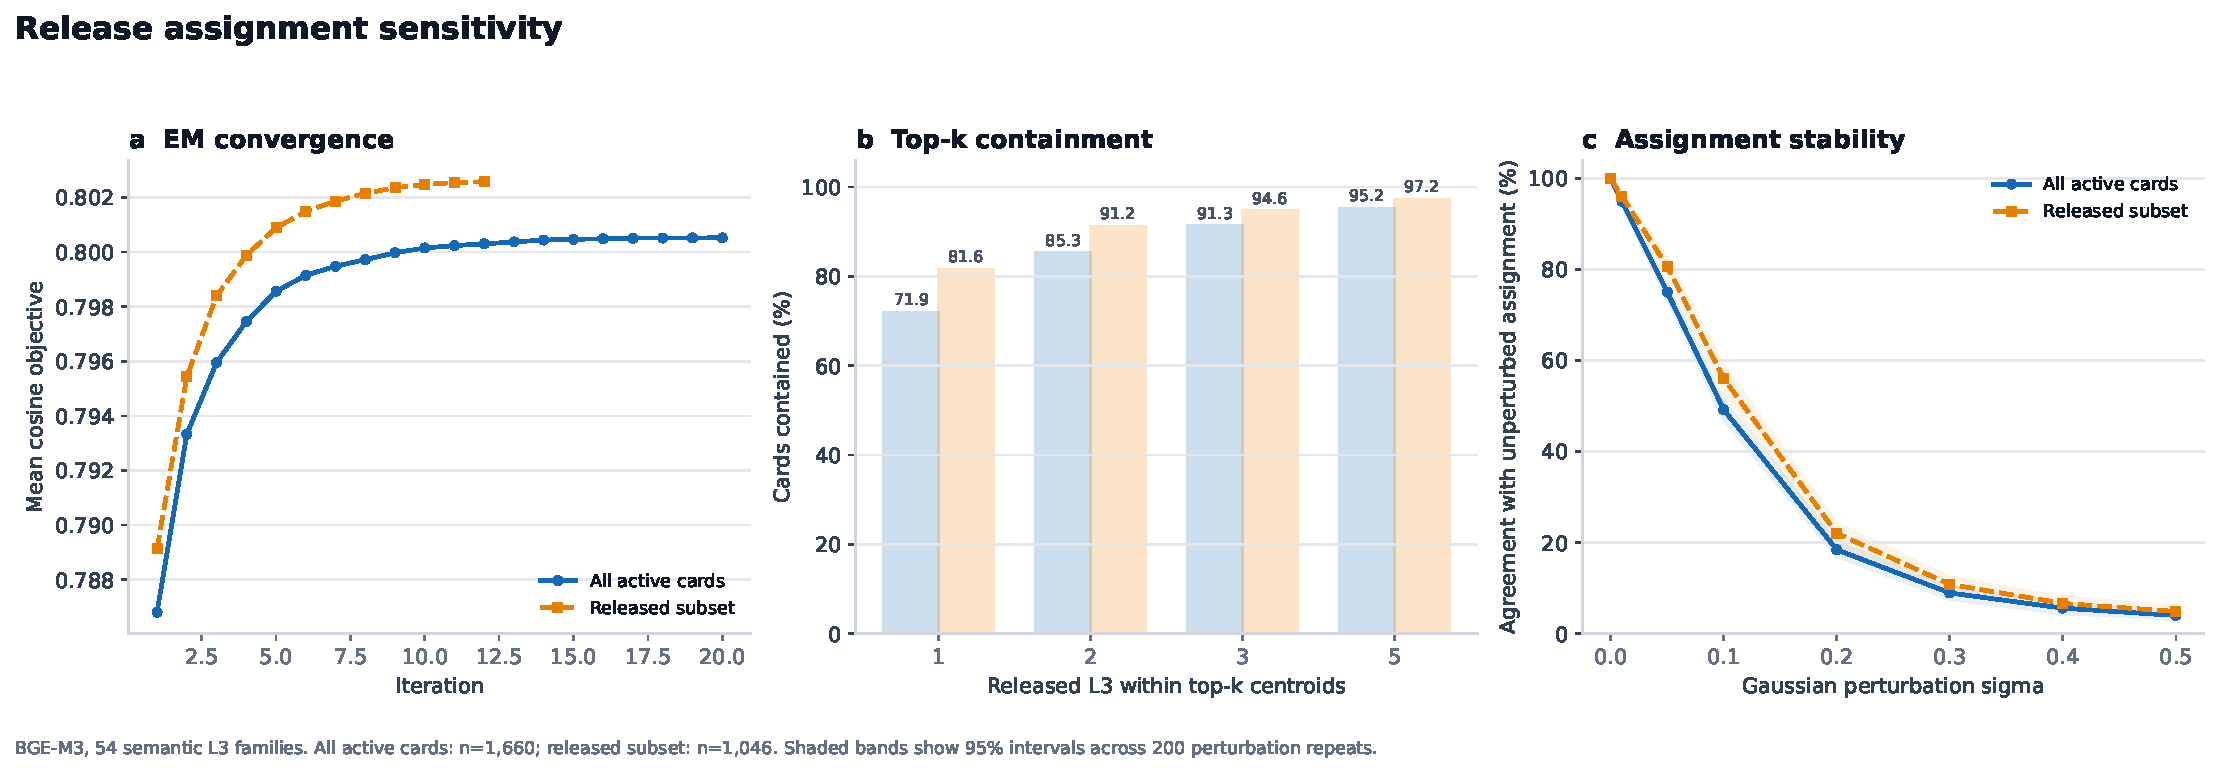
\includegraphics[width=\textwidth]{../validation/v2.18.0-rc/hold_sensitivity_bge_m3/release_assignment_sensitivity_3panel.pdf}
\caption{전체 활성 카드와 공개 확정 부분집합의 수렴성, Top-$k$ 일치율 및
Gaussian perturbation 안정성. 음영은 200회 반복의 95\% 구간이다.}
\end{figure}

\section{재현성 관리}

\begin{table}[H]
\centering
\caption{고정된 재현성 사양}
\small
\begin{tabularx}{\linewidth}{L{0.27\linewidth}Y}
\toprule
항목 & 고정값 \\
\midrule
릴리스 & v2.18.0-rc, 밀봉된 v2.17.2 입력에서 생성 \\
임베딩 모델 & BAAI/bge-m3, 정규화 1,024차원 \\
매핑 시드 & 20260725 \\
검증 시드 & 20260723 \\
최대 매핑 반복 & 30회, 변경 0건에서 조기 종료 \\
순열검정 & 5,000회 \\
노이즈 검정 & $\sigma\in\{0,0.01,0.05,0.10,0.20,0.30,0.40,0.50\}$, 각 200회 \\
카드 입력 해시 & \texttt{\seqsplit{dff3f3269a1ed8575f409923ca0c3db1aca14931259b567abeefa12da2229acf}} \\
계층 입력 해시 & \texttt{\seqsplit{76156ee383cbbf84870989f2036f0a1de6f031308fd0b9f9d5f4b821f0450050}} \\
카드 임베딩 해시 & \texttt{\seqsplit{8f99380ef026730105624d5103a37fea20ceb4816d2c5cace33b2e8c764c19d8}} \\
L3 시드 해시 & \texttt{\seqsplit{5ead12763d624a8e6d92dbb82536e18710d66c1670107c1d7d3c6e2ff18f6615}} \\
\bottomrule
\end{tabularx}
\end{table}

릴리스 빌드는 계층 이동표, 카드별 변경 이력, 반복 추적값, 임계값 판단 및
콘텐츠 해시를 기록한다. 자동 검사는 등록 ID 1,711개, 활성 카드 1,660개,
통합 이력 51개, 의미 L3 54개, 도메인별 수치, 의미 공간 노드 수 및 경로
무결성을 확인한다. Taxonomy Explorer와 Semantic Space는 브라우저 smoke
test와 console error 검사를 수행한다. PDF는 컴파일 후 페이지 렌더링과
시각 검수를 실시한다.

\section{해석과 한계}

이 분류체계는 정책 목적을 반영한 의미 분할이며, 모든 리스크에 자연적인 단일
부모가 존재한다는 가정이 아니다. 일부 L4는 복수 메커니즘을 포함해 여러 L3와
가까울 수 있으므로 Top-1과 함께 Top-$k$ 결과를 제시한다. 의미 유사도는 인과적
전파, 발생확률 또는 심각도를 의미하지 않는다. Physical 고정 경로는 안정적인
참조 집합이지만 독립적인 예측 집합은 아니다. 신규 사회적 파급 L3와 구조 이동
카드는 후속 휴먼 평가가 필요하다.

\section{결론}

현행 분류체계는 등록 ID 1,711개, 활성 L4 카드 1,660개, 의미 L2 3개, 의미 L3
54개로 구성된다. L3는 General 33개, Agentic 6개, Physical 15개다. 본 보고서의
표와 그래프는 동일한 활성 카드 스냅샷을 사용하며, 홈페이지 주 경로와 의미 검토
경로를 구분한다. 고정된 모델 입력, 난수 시드, 콘텐츠 해시, 반복 이력 및
불변조건 검사를 통해 매핑과 검증을 재현할 수 있다. 현행 결과는 휴먼 평가와
후속 릴리스 결정을 위한 기준선이며, 의미 유사도를 정답으로 간주하지 않는다.

\end{document}
